\documentclass[12pt]{article}
\usepackage[utf8]{inputenc}
\usepackage{amsmath}
\usepackage{amssymb}
\usepackage{hyperref}
\usepackage{verbatim}
\usepackage{graphicx}
\usepackage{xparse}
\usepackage{physics}

\usepackage{listings}
\usepackage{xcolor}

\definecolor{codegreen}{rgb}{0,0.6,0}
\definecolor{codegray}{rgb}{0.5,0.5,0.5}
\definecolor{codepurple}{rgb}{0.58,0,0.82}
\definecolor{backcolour}{rgb}{1,1,1}

\lstdefinestyle{mystyle}{
    backgroundcolor=\color{backcolour},   
    commentstyle=\color{codegreen},
    keywordstyle=\color{magenta},
    numberstyle=\tiny\color{codegray},
    stringstyle=\color{codepurple},
    basicstyle=\ttfamily\footnotesize,
    breakatwhitespace=false,         
    breaklines=true,                 
    captionpos=b,                    
    keepspaces=true,                 
    numbers=left,                    
    numbersep=5pt,                  
    showspaces=false,                
    showstringspaces=false,
    showtabs=false,                  
    tabsize=2
}

\lstset{style=mystyle}

\title{Mandatory Assignment 2\\Fys4130 - Statistical Mechanics}
\author{Daniel Johan Aarstein}

\begin{document}
\maketitle
\section*{Exercise 1}
\textbf{a)} \\
For our system of $L$ spins on a 1D chain with periodic boundary conditions we
have the following Hamiltonian

\begin{align*}
    H = -J\sum_{i=0}^{L-1}\delta_{\sigma_i, \sigma_{i+1}}
\end{align*}

where each spin, $\sigma$, can take the values $\{0, 1, 2\}$. \\
As the Hamiltonian is known, the partiton function is given by

\begin{align*}
    Z &= \sum_{\{\sigma\}}e^{-\beta H} \\
    &= \sum_{\{\sigma\}}e^{\beta J \sum_{i=0}^{L-1}\delta_{\sigma_i,
    \sigma_{i+1}}} \\
    Z &= \sum_{\{\sigma\}}\prod_{i=0}^{L-1}e^{\beta J \delta_{\sigma_i,
    \sigma_{i+1}}}
\end{align*}

where $\{\sigma\}$ denotes all possible spin configurations which can take
place in the system. This is equivalent to stating

\begin{align*}
    \sum_{\{\sigma\}} = \sum_{\sigma_0}\sum_{\sigma_1}\dots\sum_{\sigma_{L-1}}
\end{align*}

Note that for each $i$ in the product there are nine different combinations of
spins, three for each. These combinations can be written as a matrix, and in
turn, the entire exponential factor can be written as a so-called \textit{Transfer
Matrix}. \\
We have
\begin{align*}
    T = e^{\beta J\begin{bmatrix}1&0&0\\0&1&0\\0&0&1\end{bmatrix}}
    = \begin{bmatrix}e^{\beta J}&1&1 \\ 1&e^{\beta J}&1 \\ 1&1&e^{\beta J} \end{bmatrix}
\end{align*}

Let then $T\qty(\sigma_i, \sigma_j)$ indicate element $\qty(\sigma_i,
\sigma_j)$ of the matrix.\\
Example: $\sigma_i = 1$, $\sigma_j = 2$ gives $T(\sigma_i, \sigma_j) = T_{1, 2}
= 1$ where the indexing starts at zero.\\
\\
Note that the transfer matrix is constant throughout the entire system as the
Hamiltonian is constant. By diagonalizing the transfer matrix (wolfram
alpha was used) the following decomposition is obtained
\begin{align*}
    T &= VDV^{-1} \\
    &= \begin{bmatrix}-1&-1&1\\0&1&1\\1&0&1\end{bmatrix}
    \begin{bmatrix}e^{\beta J}-1&0&0\\0&e^{\beta J}-1&0\\0&0&e^{\beta
    J}+2\end{bmatrix}
    \begin{bmatrix}-1/3&-1/3&2/3\\-1/3&2/3&-1/3\\1/3&1/3&1/3\end{bmatrix}\\
    &= \frac{1}{3}\begin{bmatrix}-1&-1&1\\0&1&1\\1&0&1\end{bmatrix}
    \begin{bmatrix}e^{\beta J}-1&0&0\\0&e^{\beta J}-1&0\\0&0&e^{\beta
    J}+2\end{bmatrix} \begin{bmatrix}-1&-1&2\\-1&2&-1\\1&1&1\end{bmatrix}
\end{align*}

We may now rewrite the partition function as a series of sums over the product
of transfer matrices.

\begin{align*}
    Z &= \sum_{\{\sigma\}} \prod_{i=0}^{L-1}T\qty(\sigma_i, \sigma_{i+1}) \\
    &= \sum_{\sigma_0}\sum_{\sigma_1}\dots\sum_{\sigma_{L-1}}T\qty(\sigma_0,
    \sigma_1)T(\sigma_1, \sigma_2)\dots T\qty(\sigma_L-1, \sigma_0)
\end{align*}
Where the last matrix element is a consequence of the periodic boundary
    conditions.

From linear algebra it is known that an element in a matric product can be
written as
\begin{align*}
    \qty(AB)_{i,j} = \sum_k A_{i, k}B_{k, j}
\end{align*}

Hence the partition function is given by
\begin{align*}
    Z &= \sum_{\sigma_0}\sum_{\sigma_1}\dots\sum_{\sigma_{L-2}}
    T\qty(\sigma_0, \sigma_1)T\qty(\sigma_1, \sigma_2)\dots T\qty(\sigma_{L-3},
    \sigma_{L-2}) \underbrace{\sum_{\sigma_{L-1}}T\qty(\sigma_{L-2},
    \sigma_{L-1})T\qty(\sigma_{L-1}, \sigma_0)}_{T^2\qty(\sigma_{L-2},
    \sigma_0)} \\
    &= \sum_{\sigma_0}\sum_{\sigma_1}\dots\sum_{\sigma_{L-3}}T\qty(\sigma_0,
    \sigma_1)T\qty(\sigma_1, \sigma_2)\dots T\qty(\sigma_{L-4}, \sigma_{L-3})
    \underbrace{\sum_{\sigma_{L-2}}T\qty(\sigma_{L-3},
    \sigma_{L-2})T^2\qty(\sigma_{L-2}, \sigma_0)}_{T^3\qty(\sigma_{L-3},
    \sigma_0)} \\
    &\vdots \\
    Z &= \sum_{\sigma_0}T^L\qty(\sigma_0, \sigma_0)
\end{align*}
This final expression is the sum over the diagonal elements of the matrix
    $T^L$, also known as its trace. Thus we have
\begin{align*}
    Z = \Tr(T^L)
\end{align*}
Since $T$ is a diagonalizable matrix, $T^L = VD^LV^{-1}$. Since the trace
operation is invariant under cyclic permutation, we have that

\begin{align*}
    Z &= \Tr(T^L) = \Tr(VD^LV^{-1}) = \Tr(V^{-1}VD^L) = \Tr(D^L) \\
    &= \Tr\qty(\begin{bmatrix}\qty(e^{\beta J}-1)^L&0&0 \\ 0&\qty(e^{\beta
    J}-1)^L&0 \\ 0&0&\qty(e^{\beta J} + 2)^L\end{bmatrix}) \\
    Z &= 2\qty(e^{\beta J}-1)^L + \qty(e^{\beta J} + 2)^L
\end{align*}

With an expression for the partition function we can calculate the internal
energy of the system.
\begin{align*}
    U &= -\pdv{\ln Z}{\beta} \\
    &= -\frac{2LJe^{\beta J}\qty(e^{\beta J}-1)^{L-1} + LJe^{\beta J}\qty(e^{\beta
    J}+2)^{L-1}}{2\qty(e^{\beta J}-1)^L + \qty(e^{\beta J} + 2)^L} \\
    U &= -\frac{LJe^{\beta J}\qty[2\qty(e^{\beta J}-1)^{L-1} + \qty(e^{\beta J} +
    2)^{L-1}]}{2\qty(e^{\beta J}-1)^L + \qty(e^{\beta J} + 2)^L}
\end{align*}

Using $\qty(e^{\beta J} - 1) = e^{\beta J}\qty(1 - e^{-\beta J})$ and
$\qty(e^{\beta J}+2) = e^{\beta J}\qty(1 + 2e^{-\beta J})$ the above
expression becomes

\begin{align*}
    U &= -\frac{LJe^{L\beta J}\qty[2\qty(1-e^{-\beta J})^{L-1} + \qty(1 +
    2e^{-\beta J})^{L-1}]}{e^{L\beta J}\qty[2\qty(1-e^{-\beta J})^L + \qty(1 +
    2e^{-\beta J})^L]} \\
    U &= -LJ\frac{2\qty(1-e^{-\beta J})^{L-1} + \qty(1 +
    2e^{-\beta J})^{L-1}}{2\qty(1-e^{-\beta J})^L + \qty(1 +
    2e^{-\beta J})^L}
\end{align*}

For high temperatures $\beta \rightarrow 0$, $\qty(1-e^{-\beta J}) \Rightarrow
0$ and $(1 + 2e^{-\beta J}) \Rightarrow 3$. The energy then becomes
\begin{align*}
    U_{High} = -LJ\frac{3^{L-1}}{3^L} = \frac{-LJ}{3}
\end{align*}

For low temperatures $\beta \rightarrow \infty$, $\qty(1-e^{-\beta J})
\Rightarrow 1$ and $\qty(1 + 2e^{-\beta J}) \Rightarrow 1$. The energy then
becomes
\begin{align*}
    U_{Low} = -LJ\frac{2 + 1}{2 + 1} = -LJ
\end{align*}

Explain these limiting behaviors
\\
\textbf{b)} \\

Moving on to the mean magnetization, we have

\begin{align*}
    \expval{m} &= \expval{\frac{1}{N}\sum_{j=0}^{N-1}m_j} \\
    &= \frac{1}{N}\sum_{j=0}^{N-1}\expval{m_j}
\end{align*}

Since this sum is finite the above expression is valid. \\
The problem is now reduced to finding the expectation value for each of the
local "magnetizations". Using the partition funciton as the probability
distribution and the provided definiton of the local magnetization, we have

\begin{align*}
    \expval{m_j} &=
    \frac{1}{Z}\sum_{\{\sigma\}}e^{i\frac{2\pi}{3}\sigma_j}\prod_{i=0}^{L-1}
    e^{\beta J \delta_{\sigma_i, \sigma_{i+1}}}
\end{align*}
Using a similar approach to finding the partition function, this can be
expanded as a sum over the product of multiple transfer matrices.

\begin{align*}
    \expval{m_j} &= \frac{1}{Z}\sum_{\sigma_0}\sum_{\sigma_1}\dots\sum_{\sigma_{L-1}}
    e^{i\frac{2\pi}{3}\sigma_j} T\qty(\sigma_0, \sigma_1)T\qty(\sigma_1,
    \sigma_2)\dots T\qty(\sigma_{L-1},\sigma_0) \\
    &= \frac{1}{Z}\sum_{\sigma_j}e^{i\frac{2\pi}{3}\sigma_j}
    \sum_{\sigma_0}\sum_{\sigma_1}\dots\sum_{\sigma_{j-1}}\sum_{\sigma_{j+1}}\dots
    \sum_{\sigma_{L-1}}T\qty(\sigma_0, \sigma_1)T\qty(\sigma_1, \sigma_2) \dots
    T\qty(\sigma_{L-1}, \sigma_0) \\
    &= \frac{1}{Z}\sum_{\sigma_j}e^{i\frac{2\pi}{3}\sigma_j}
    \sum_{\sigma_0}\sum_{\sigma_1}\dots\sum_{\sigma_{j-1}}T\qty(\sigma_0,
    \sigma_1)T\qty(\sigma_1, \sigma_2)\dots T\qty(\sigma_{j-1}, \sigma_j) \\
    &\qquad\sum_{\sigma_{j+1}}\dots\sum_{\sigma_{L-1}} T\qty(\sigma_j,
    \sigma_{j+1})T\qty(\sigma_{j+1}, \sigma_{j+2})\dots T\qty(\sigma_{L-1},
    \sigma_0) \\
    &=\frac{1}{Z}\sum_{\sigma_j}e^{i\frac{2\pi}{3}\sigma_j}
    \sum_{\sigma_0}T^{j}\qty(\sigma_0, \sigma_j)T^{L-j}\qty(\sigma_j,
    \sigma_0)
\end{align*}

Where is has been used that
$\sum_{\sigma_1}\dots\sum_{\sigma_{j-1}}T\qty(\sigma_0,\sigma_1)\dots
T\qty(\sigma_{j-1}, \sigma_j) = T^{j}\qty(\sigma_0, \sigma_j)$ and 
$\sum_{\sigma_{j+1}}\dots\sum_{\sigma_{L-1}} T\qty(\sigma_j,
\sigma_{j+1})\dots T\qty(\sigma_{L-1},\sigma_0) = T^{L-j}\qty(\sigma_j,
\sigma_0)$. \\
Since $T^{j}\qty(\sigma_0, \sigma_j)$ and
$T^{L-j}\qty(\sigma_j,\sigma_0)$ are elements of matrices, they are simply
numbers, and thus commute. The order of multiplication can then be switched
giving us

\begin{align*}
    \expval{m_j} &= \frac{1}{Z}\sum_{\sigma_j}e^{i\frac{2\pi}{3}\sigma_j}
    \sum_{\sigma_0}T^{L-j}\qty(\sigma_j, \sigma_0)T^{j}\qty(\sigma_0,
    \sigma_j) \\
    \expval{m_j} &= \frac{1}{Z}\sum_{\sigma_j}e^{i\frac{2\pi}{3}\sigma_j}T^L\qty(\sigma_j,
    \sigma_j)
\end{align*}

This final sum will only take the diagonal elements of the matrix $T^L$ which
can be calculated by $T^L = VD^LV^{-1}$ where $V$ and $D$ are the eigenvector
and eigenvalue matrices from exercise a). Carrying out the full calculation;
%shows that all the diagonal elements are equal;
\begin{align*}
    T^L &= VD^LV^{-1} \\
    &= \frac{1}{3} \begin{bmatrix}-1&-1&1\\0&1&1\\1&0&1\end{bmatrix}
        \begin{bmatrix}\qty(e^{\beta J}-1)^L&0&0\\0&\qty(e^{\beta J}-1)^L&0
        \\0&0&\qty(e^{\beta J}+2)^L\end{bmatrix}
        \begin{bmatrix}-1&-1&2\\-1&2&-1\\1&1&1\end{bmatrix} \\
    &= \frac{1}{3}
    \begin{bmatrix}2\qty(e^{\beta J}-1)^L + \qty(e^{\beta J}+2)^L &
    -\qty(e^{\beta J}-1)^L + \qty(e^{\beta J}+2)^L & -\qty(e^{\beta J}-1)^L +
    \qty(e^{\beta J}+2)^L \\ -\qty(e^{\beta J}-1)^L + \qty(e^{\beta J}+2)^L &
    2\qty(e^{\beta J}-1)^L + \qty(e^{\beta J}+2)^L & -\qty(e^{\beta J}-1)^L +
    \qty(e^{\beta J}+2)^L \\ -\qty(e^{\beta J}-1)^L + \qty(e^{\beta J}+2)^L &
    -\qty(e^{\beta J}-1)^L + \qty(e^{\beta J}+2)^L & 2\qty(e^{\beta J}-1)^L + \qty(e^{\beta J}+2)^L\end{bmatrix}
\end{align*}

Which gives

\begin{align*}
    T^L\qty(\sigma_j, \sigma_j) &= \frac{2\qty(e^{\beta J}-1)^L + \qty(e^{\beta
    J}+2)^L}{3} \quad \forall \quad \sigma_j
\end{align*}

Thus

\begin{align*}
    \expval{m_j} &=
    \frac{2\qty(e^{\beta J}-1)^L + \qty(e^{\beta
    J}+2)^L}{3Z}\sum_{\sigma_j}e^{i\frac{2\pi}{3}\sigma_j} \\
    &= \frac{2\qty(e^{\beta J}-1)^L + \qty(e^{\beta
    J}+2)^L}{3Z} \underbrace{\qty(1 + e^{i\frac{2\pi}{3}} +
    e^{i\frac{4\pi}{3}})}_{=0} \\
    \expval{m_j} &= 0
\end{align*}

From this it follows that $\expval{m} = \frac{1}{N}\sum_j\expval{m_j} = 0$.
\\
\textbf{c)} \\

Starting of by noting that the correlation function $C(r)$ is nothing else than
the covariance between the complex conjugate magnetization at site zero and at
a site distance $r$ from site zero.
Again using the partition function in constructing the probability distribution
as well as the definition of the covariance, we have that

\begin{align*}
    C(r) = \text{Cov}(m_0^*, m_r) &= \frac{1}{Z}\sum_{\{\sigma\}}\prod_i e^{\beta
    J\delta_{\sigma_i, \sigma_{i+1}}}\qty(m_0^* - \expval{m_0^*})\qty(m_r -
    \expval{m_r})
\end{align*}

Knowing that the expectation value for magnetization is zero, we have

\begin{align*}
    C(r) &= \frac{1}{Z}\sum_{\{\sigma\}}\prod_iT\qty(\sigma_i, \sigma_{i+1})
    m_0^*m_r
\end{align*}

The magnetization is only dependent on the spins at sites $0$ and $r$, so these
sums can be extracted. Using the provided definition, $m_j \equiv 
e^{i\frac{2\pi}{3}\sigma_j}$, we have

\begin{align*}
    C(r) &=
    \frac{1}{Z}\sum_{\sigma_0}e^{-i\frac{2\pi}{3}\sigma_0}\sum_{\sigma_r}
    e^{i\frac{2\pi}{3}\sigma_r} \sum_{\sigma_1}\dots
    \sum_{\sigma_{r-1}} T\qty(\sigma_0, \sigma_1)\dots
    T\qty(\sigma_{r-1}, \sigma_r) \\ &\qquad \sum_{\sigma_{r+1}}\dots
    \sum_{\sigma_{L-1}}T\qty(\sigma_r, \sigma_{r+1}) \dots T\qty(\sigma_{L-1},
    \sigma_0) \\
    &= \frac{1}{Z}\sum_{\sigma_0}e^{-i\frac{2\pi}{3}\sigma_0}
    \sum_{\sigma_r}e^{i\frac{2\pi}{3}\sigma_r} T^r\qty(\sigma_0,
    \sigma_r)T^{L-r}\qty(\sigma_r, \sigma_0)
\end{align*}

The elements in the matrices $T^r$ and $T^{L-r}$ are known, and we can simply
carry out the calculation

\begin{align*}
    C(r) &= \frac{1}{Z}\sum_0e^{-i\frac{2\pi}{3}\sigma_0}\qty(
    T^r\qty(\sigma_0, 0)T^{L-r}\qty(0, \sigma_0) +
    e^{i\frac{2\pi}{3}}T^r\qty(\sigma_0, 1)T^{L-r}\qty(1, \sigma_0) +
    e^{i\frac{4\pi}{3}}T^r\qty(\sigma_0, 2)T^{L-r}\qty(2, \sigma_0)) \\
    &= \frac{1}{Z} [T^r(0, 0)T^{L-r}(0, 0) + e^{i\frac{2\pi}{3}}T^r(0,
    1)T^{L-r}(1, 0) + e^{i\frac{4\pi}{3}}T^r(0, 2)T^{L-r}(2, 0) \\
    &\qquad e^{-i\frac{2\pi}{3}}T^r(1, 0)T^{L-r}(0, 1) + T^r(1, 1)T^{L-r}(1, 1)
    + e^{i\frac{2\pi}{3}}T^r(1, 2)T^{L-r}(2, 1) \\
    &\qquad e^{-i\frac{4\pi}{3}}T^r(2, 0)T^{L-r}(0, 2) +
    e^{-i\frac{2\pi}{3}}T^r(2, 1)T^{L-r}(1, 2) + T^r(2, 2)T^{L-r}(2, 2)]
\end{align*}

Every diagonal element is the same, and every off-diagonal element is the same.
Lets therefore introduce

\begin{align*}
    \chi &= T^r(\sigma_i, \sigma_i)T^{L-r}(\sigma_i,
    \sigma_i)\\ 
    &= \frac{1}{9}\qty(4\qty(e^{\beta J}-1)^L + \qty(e^{\beta J}+2)^L + 2\qty(e^{\beta
J}-1)^r\qty(e^{\beta J}+2)^{L-r} + 2\qty(e^{\beta J}-1)^{L-r}\qty(e^{\beta
J}+2)^r)
\end{align*}

and 
\begin{align*}
    \xi &= T^r(\sigma_i, \sigma_j)T^{L-r}(\sigma_i, \sigma_j)\\
    &=\frac{1}{9}\qty(\qty(e^{\beta J}-1)^L + \qty(e^{\beta J}+2)^L-
    \qty(e^{\beta J}-1)^r\qty(e^{\beta J}+2)^{L-r} - \qty(e^{\beta
    J}-1)^{L-r}\qty(e^{\beta J}+2)^r)
\end{align*}

The correlationfunction is then

\begin{align*}
    C(r) &= \frac{1}{Z}[3\chi + \xi\underbrace{\qty(2e^{i\frac{2\pi}{3}} + 2e^{-i\frac{2\pi}{3}} +
    e^{i\frac{4\pi}{3}} + e^{-i\frac{4\pi}{3}})}_{= -3}] \\
    &= \frac{3}{Z}\qty(\chi - \xi)
\end{align*}

From a) we have that $Z = 2\qty(e^{\beta J}-1)^L + \qty(e^{\beta J}+2)^L$, which
in total gives us

\begin{align*}
    C(r) &= \frac{\qty(e^{\beta J}-1)^L + \qty(e^{\beta J}-1)^r\qty(e^{\beta
    J}+2)^{L-r} + \qty(e^{\beta J}-1)^{L-r}\qty(e^{\beta J}+2)^r}{2\qty(e^{\beta J}-1)^L + \qty(e^{\beta J}+2)^L}
\end{align*}

"Is this correct?" - Daniel, 24 år \\
"Yes."  - João, 21 anos

\newpage
\section*{Exercise 2}

\textbf{a)} \\
\\
\noindent All code and relevant txt-files can be found in the following
Github-repository; \url{https://github.com/danaars/FYS4130}. \\
\\
\textbf{b)} \\
\\
For the one-dimensional case with periodic boundary conditions the following
correlations were computed by using
\begin{align*}
    C(r) = \expval{m_0^*m_r} - \expval{m_0^*}\expval{m_r}
\end{align*}

The following results are obtained with 100000 Monte Carlo Cycles.\\
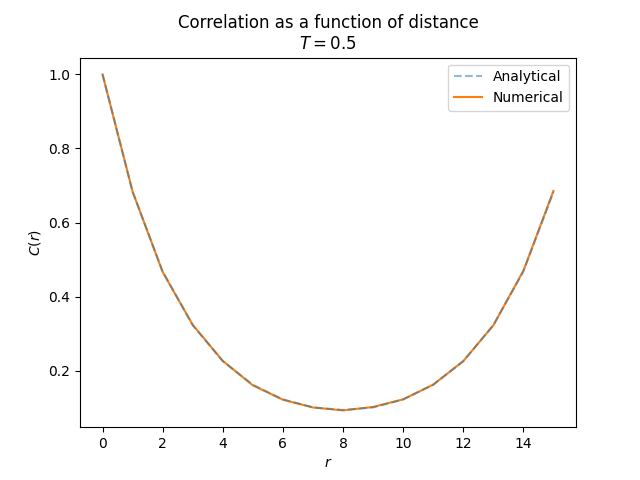
\includegraphics[width = \textwidth]{hTcorr.png} \\
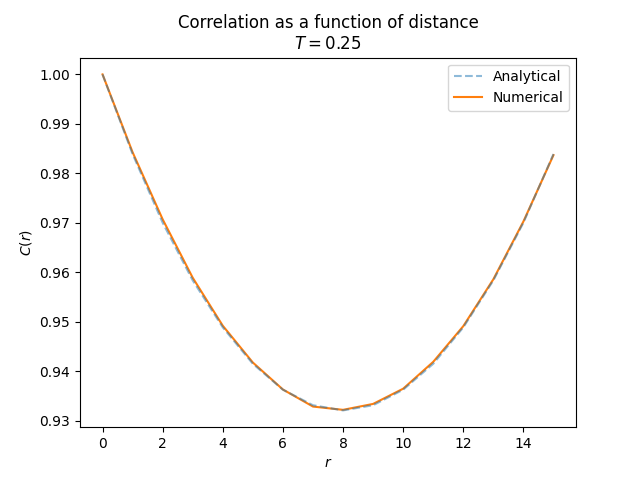
\includegraphics[width = \textwidth]{lTcorr.png}
\\
Note that the correlation is high 
\\ \\
\textbf{c)} \\
\\
\noindent For this part, two results were obtained. The only difference in the
calculation (i.e. code) is illustrated in the following lines of pseudo code

\begin{lstlisting}[language=C++]
if (spin[x][y] == 0){
    // Case A
    spin[x][y] = 1;
    // or
    // Case B
    spin[x][y] = (r < 0.5) ? 1:2;
}
\end{lstlisting}

Case A simply changes the spin at location $(x, y)$ from $0$ to $1$ with
probability $1$. Case B is perhaps more realistic for a physical process, in
that the spin at location $(x, y)$ changes to one of the other possible spins, each with probability
$0.5$. \\
For $L=16$ the real part of the average magnetization per site is given by the following
plots. \\
Case A:\\
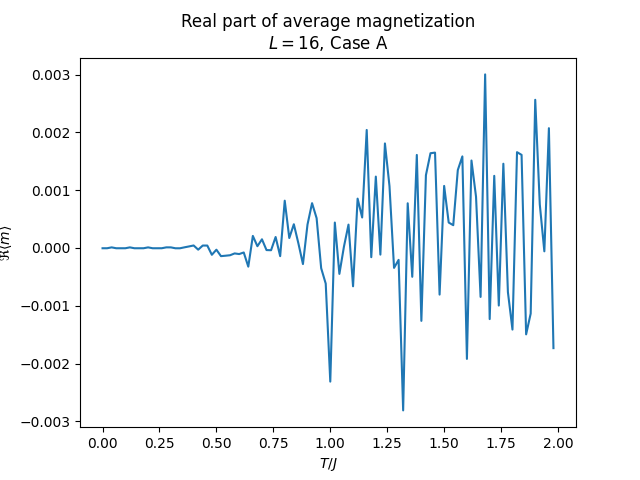
\includegraphics[width = \textwidth]{ram.png}\\
Case B: \\
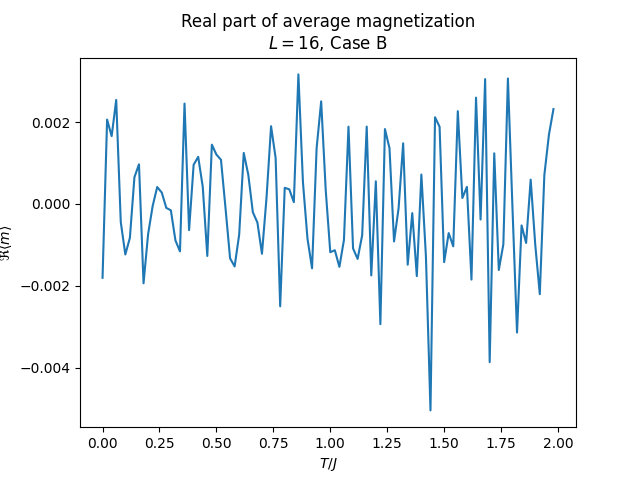
\includegraphics[width = \textwidth]{r_ram.png}\\

Note that for case A (the less random one) the real part of the average
magnetization is close to zero untill the temperature reaches about $T = 0.6$.
This, however, is not the case in case B. Here the real part of the average
magnetization fluctuates more or less randomly irregardless of temperature.\\
For the rest of the exercise, calculations have been carried out with the case
A syntax.\\
\\
\textbf{d)} \\
\\
For $L = 16$ the average of the absolute magnetization squared is as follows \\
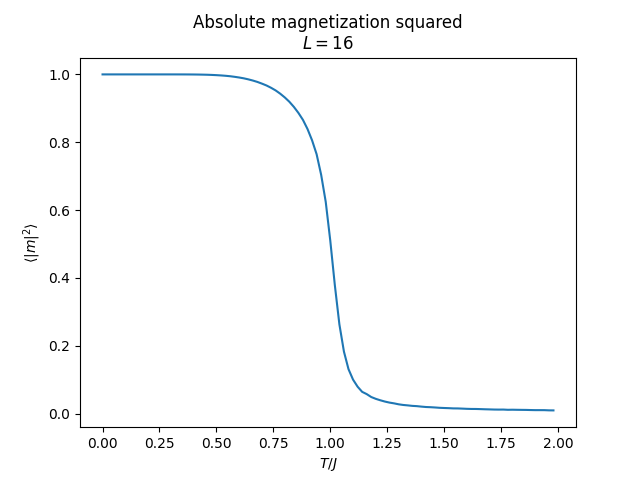
\includegraphics[width = \textwidth]{ams.png} \\
\\
For $T/J = 0$, $\expval{\abs{m}^2} = 1$, for $T/J \to \infty$,
$\expval{\abs{m}^2} = 0$. \\
\\
\textbf{e)} \\
\\
\textbf{f)} \\
\\
For systems of sizes $L = {8, 16, 32}$ the following results of $\Gamma$ were
obtained\\
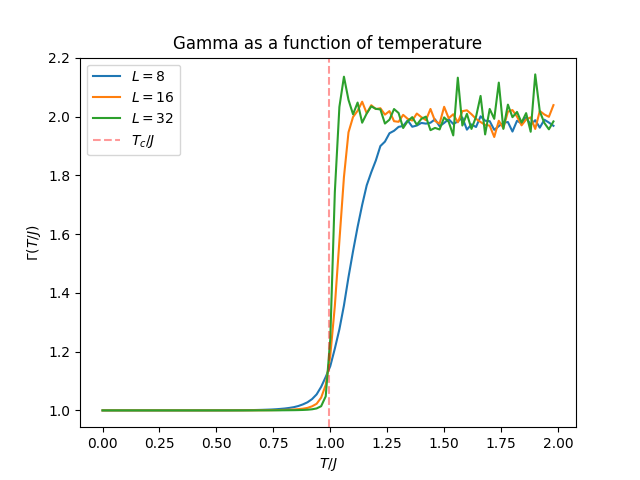
\includegraphics[width = \textwidth]{gamma.png}\\
zooming in we have that \\
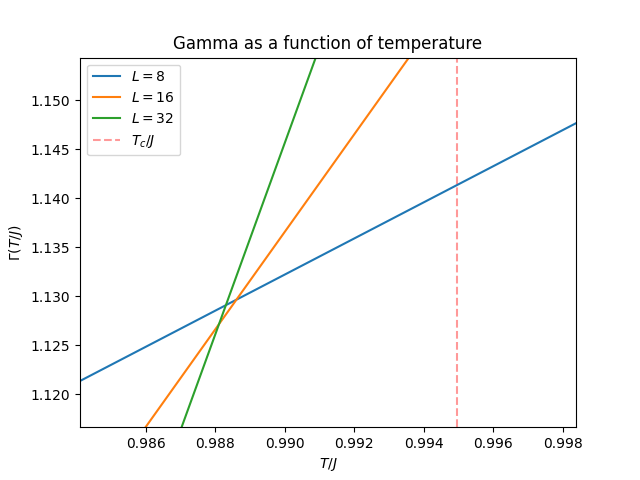
\includegraphics[width = \textwidth]{gamma_zoom.png}\\
The graphs are 100 calculations for $T/J$ from $0$ to $2$. That gives $\Delta
T/J = \frac{2}{100} = 0.02$ The graphs cross at a distance smaller than $\Delta
T/J$ from the theoretical $T_c/J$. For a finer resolution it then might be the
case that the graphs cross at exactly $T_c/J$, as they should in theory. \\
If the graphs dont cross in a single point something must be wrong with our
assumption that the function $\Gamma$ is a function of only $t$ and $L^{-1}$.

\end{document}
